% #############################################################################
% This is Chapter 6
% !TEX root = ../main.tex
% #############################################################################
% Change the Name of the Chapter i the following line
\fancychapter{Evaluation}
% The following line allows to ref this chapter
\label{chap:evaluation}

After completing the last cycle of development, a set of users tested the Sterio system, in order to gather quantitative and qualitative usability metrics to assure that our platform meets both users’ needs and our set goals. We start by presenting the methodology used, followed by the description of the tasks defined for the test sessions, justifying, for each, what we want to conclude by asking users to do it. We finally present the analysis of the test results and the workload estimated for the prototype, as well as the conclusions that we were able to get from the results.


% #############################################################################
\section{Methodology}

When a final functional prototype of the platform with a working set of features was completed, a group of 26 potential users tested the system. This set of users were of distinct ages, occupations, socio-economical backgrounds, and audio media consuming habits. From these users, 21 haven't participated in either of the previously-mentioned user research (described in Chapter ~\ref{chap:userresearch}) and speed dating activities (examined in Chapter ~\ref{sec:speeddating}), while the remaining 5 have participated in these ventures.

This evaluation was conducted to assess the success of the final prototype and to check that a standard was upheld, which is a process known as summative evaluation. ~\cite{Preece2015, Courage2005} The same list of tasks and protocols were presented to each user, and their performance was evaluated mainly through qualitative measures, as we want to deeply understand the type of experience that is created while users indulge in the platform, as well as insights, findings, and anecdotes about the experience of the user.

To help us steer the session, and to keep all gatherings as cohesive and alike as possible, the first step was to write a protocol guide, shown in Appendix CENAS. All sessions were conducted in a physical location, where several measures were taken to comply with health and safety guidelines as a response to the COVID-19 pandemic. For instance, the researcher and the user were seated at least 2 meters apart from each other, complying with the social distancing rules. All surfaces — including the provided smartphone on where the prototype was tested — were disinfected before and after the session. Users were required to utilize hand sanitizer when entering and leaving the room and were also asked to bring their smartphone so that they could fill out the necessary survey forms. 

We planned each testing session to be divided into 3 distinct segments, which we will describe in the following subsections.

\subsection{Introduction, Informed Consent Form, and Initial Survey}

After the user's arrival to the testing room, the facilitator invited them to sit in a comfortable way. In front of them, three items were displayed: a smartphone with the loaded Sterio system; a sheet containing a set of QR codes that redirects users to the necessary survey forms; and a helping sheet that contains extra information regarding the tasks.

In order to contextualize each user on what the purposes of the testing were, an introduction was read by the research. Then, users were asked to carefully read and sign an informed consent form (presented in Appendix CENAS. Finally, by presenting them an initial survey (showcased in Appendix CENAS), we collected demographic information and other relevant details of the user, such as if they had any visual or hearing conditions, as well as their general audio media consumption habits.

\subsection{User Training and Task Protocol}
\label{subsub:taskprot}

After the initial remarks, the user was allowed a maximum of five minutes to explore freely the platform's four main screens. The remaining screens were not available for the users to explore in the first stage, as this could interfere with the testing results. During this period, the user could ask any questions. After they felt ready to do so, we began the testing session.

The core testing session consisted of 4 different tasks, that are further described in Section ~\ref{sub: tasks}. Each task followed a specific protocol that was transversal to all tasks. First, the researcher presented the task and gave space for the user to clarify any questions related to the disclosure of the task.

Then, after the consent of the user, the researcher started a stopwatch timer to count the time the user took to perform the task. Furthermore, the screen of the used smartphone was also recorded, to help later in the protocol. At the same time, the facilitator was paying attention to the user's actions, taking relevant notes about the usability when appropriate, and counting the number of errors (if any occurred). Beforehand, it was communicated to the user that it was not possible to express any comments nor ask any questions unless a very high level of difficulty whilst performing the task was detected.

Right after the conclusion of the task, the user is asked to fill out a post-task survey that evaluates quantitatively the general experience, usability, and difficulties felt by the user. This survey is showcased in Appendix CENAS.

To gather a broad dataset of qualitative data, two types of moderation to encourage each tester to share their thought process were applied: \ac{RTA}, where the moderator asks participants to retrace their steps when the session is complete, and \ac{RP}, where the researcher asks detailed and relevant questions after the fact.

Regarding \ac{RTA}, a video replay of the user's actions was shown, so that it was easier for them to recall and express their line of thought as they performed the task. The researcher took relevant notes as the user expressed their reasoning.

Lastly, users were asked specific questions about their thoughts and action, such as "What would you do differently?" and were encouraged to elaborate on their responses. As the user was expressing comments, the researcher took relevant notes.

Each of the four tasks followed this protocol, whose duration was an average of 5 minutes per item. 

\subsection{Final Debrief}
\label{sub:final}

After the conclusion of the four tasks, users were redirected to a final survey, presented in Appendix CENAS, which was subdivided into two sections. 

The first half consisted of a \ac{SUS}, which is a simple, ten-item scale giving a global view of subjective assessments of usability [28] about the user experience with the Sterio system. We followed the guidelines established by Brooke [28]: each question had a degree of disagreement or agreement, with a range from Strongly Disagree (1) to Strongly Agree (5) respectively, from which the user could choose. Users were asked to answer each question honestly, but not too attentively.

The latter half of the final survey consisted of Microsoft's Product Reaction Cards method, which consists of a list of 118 words that might be used to describe a product. The list includes positive words like ‘Useful’ and ‘Engaging’, together with negative words, such as ‘Frustrating’ and ‘Ineffective’. Users were asked to choose up to 5 of these words, which were sorted randomly to avoid any bias.

Finally, to close the session, a short final interview with the user was conducted. These interviews allowed the participants to shed light on their experience without extra prompting. A semi-structured approach using a few predetermined questions was applied in the first stage, but afterward, the interviews took their own direction, which uncovered some very useful insights regarding our platform. As the interview was unrolled, the researcher took note of relevant aspects and observations.

% #############################################################################
\section{Tasks}
~\label{sub:tasks}

The core evaluation session consisted of 4 different tasks that allowed us to understand if our platform met our established usability goals. These tasks should not be too complex, but should be able to explore the full capabilities and features of our prototype, so that we can uncover as much detail as possible regarding the user's experience.

The complete set of four tasks is:

\begin{enumerate}
	\item Create a new station \textit{(Create)}
	\item Configure the station's blocks \textit{(Create)}
	\item Play the created station \textit{(Listen)}
	\item Share the created station \textit{(Share)}
\end{enumerate}

These tasks are focused on the defined three main user enactments on Section ~\ref{sec:userenactments} — tasks 1 and 2 for the 'Create' enactment, task 3 for the 'Listen' enactment, and task 4 for the 'Share' enactment. This setting allowed us to better understand and organize the session, as well as to steer our results and compare them with the previously discussed matter.

In the first task, users were asked to create a new station with a given name ('Feel Good'), description ('The best hits!'), cover (the first image on the gallery of the smartphone), and blocks (Spotify, Weather, and News). This was a simple task that evaluated the ease of use of the platform, as well as how quickly the user can create a fully tailored and customized station.

The second task was the most complex, as it required a lot of input from the user. Users were asked to configure the three added blocks (Spotify, Weather, and News). For the Spotify block, they were asked to select one of the 5 available playlists, which had identical duration but with a distinct set of songs to match the user's taste. In the Weather block, users were asked to select the current location, current conditions, hourly forecast, and 3-day forecast, with the periodicity set to 5 minutes. Finally, in the News block, users were asked to select the 'General', 'Health', and 'Entertainment' categories, with 6 as the number of headlines and periodicity of 5 minutes. One of our established goals was to make as simple as possible for the user to tailor and customize the station to their taste, and this task let us uncover helpful insights in this matter.

The third task was the most simple one for the user to perform but was the most critical for our study. Users were asked to play their created station and to listen carefully to its content. Then, they were asked to enter in the 'Schedule' screen of the station, as well as to find and enter the 'Now Playing' screen whilst the station was playing. Ultimately, this task gave us really important feedback on the experiences the users felt while indulging in this new listening model.

Finally, the fourth task tested our platform's social capabilities. Users were asked to enter in the 'Social' screen and follow the 'Roger Waters' profile. Then, it was simulated that such a profile was listening to a shared station, and users were asked to listen along (testing the simultaneous listening experience). Afterward, users were asked to enter the "My Day" shared station, and change the News periodicity to 4 minutes. This task allowed users to experience the social counterpart of the platform, giving us important feedback on their experience.

The execution of each of the four tasks followed the same protocol, described previously in Section ~\ref{subsub:taskprot}. Each task didn't surpass 5 minutes in performing them, which allowed us to maintain our goal of keeping the total duration of the sessions in the window of 30 to 35 minutes.

% #############################################################################
\section{Results}

In this section, we present the results obtained from the execution of the test sessions. We start by presenting the users’ characterization (sub-section 5.3.1), followed by a statistical analysis we made to compare results between tasks (sub-section 5.3.2). Then, we examine and review all the gathered qualitative data (sub-section 5.3.3). Finally, in sub-section 5.3.4, we present some conclusions regarding suggestions gathered and notes taken by observation during the test sessions with the users.

\subsection{Users’ Characterization}

A total of 26 users participated in the test sessions. From those, 15 were of ages ranging from 18 to 30, while the remaining 11 refer to ages 31 to 60. A majority of the participants were female (16 users). Aproximmatelly 54\% were employed, while the remaining 46\% were students. None of these users had a visual or hearing condition that cloud affect their performance on the testing sessions.

As for audio media consuming habits, 76.5\% of the users use a music streaming service on a daily basis, with only 5.9\% using them 'rarely'. With 81\%, Spotify is the most used streaming service, followed by YouTube which counts for 5.9\%. As for traditional terrestrial radio stations, 41.2\% of the users state that they listen to it on a weekly basis, while 17.6\% listen to them daily and just 5.9\% not listening to them at all.

\subsection{Statistical Analysis}

In this sub-section, we present the results of the statistical analysis performed over the test results. This analysis was conducted with the goal of understanding, in raw metrics, the usability of our system. We evaluated success, time taken to answer, and difficulty evaluated by the users.

\subsubsection{Duration and Number of Errors}

Table ~\ref{tab:resultstimetourist} presents the duration it took each user to perform each task, as well as the number of errors. In the same table, some statistics about those values are also presented, which show the values referring to the minimum, maximum, and average time spent executing each task, the value of the standard deviation, and the confidence interval with the confidence level of 95\%.

We decided not to count nor analyze the time the users took to perform tasks 3 and 4. These tasks involved playing a station, in which the total time of listening would depend on a variety of factors. As such, this wouldn't be an indicative value to study and take into consideration in our analysis.


\setlength{\tabcolsep}{0.5em} % for the horizontal padding
{\renewcommand{\arraystretch}{1.2}% for the vertical padding
\begin{table}
\centering
\setlength{\extrarowheight}{0pt}
\addtolength{\extrarowheight}{0pt}
\addtolength{\extrarowheight}{0pt}
\setlength{\aboverulesep}{0pt}
\setlength{\belowrulesep}{0pt}
\caption{Statistical Analysis — Duration and Number of Errors}
\label{tab:resultstimetourist}
\resizebox{\linewidth}{!}{%
\begin{tabular}{>{\hspace{0pt}}p{0.357\linewidth}|>{\centering\hspace{0pt}}p{0.136\linewidth}|>{\centering\hspace{0pt}}p{0.136\linewidth}|>{\centering\hspace{0pt}}p{0.071\linewidth}|>{\centering\hspace{0pt}}p{0.071\linewidth}|>{\centering\hspace{0pt}}p{0.071\linewidth}|>{\centering\arraybackslash\hspace{0pt}}p{0.071\linewidth}} 
\hline
\multicolumn{1}{>{\centering\hspace{0pt}}p{0.357\linewidth}|}{} & \multicolumn{2}{>{\centering\hspace{0pt}}p{0.272\linewidth}|}{\textbf{Duration (seconds)} } & \multicolumn{4}{>{\centering\arraybackslash\hspace{0pt}}p{0.284\linewidth}}{\textbf{Number of Errors}} \\ 
\hline
\multicolumn{1}{>{\centering\hspace{0pt}}p{0.357\linewidth}|}{} & \multicolumn{6}{>{\centering\arraybackslash\hspace{0pt}}p{0.556\linewidth}}{\textbf{Tasks} } \\ 
\hhline{-------}
\rowcolor[rgb]{0.851,0.851,0.851}  \textbf{Users}  & \multicolumn{1}{>{\centering\hspace{0pt}}p{0.136\linewidth}}{\textbf{T1} } & \textbf{T2}  & \multicolumn{1}{>{\centering\hspace{0pt}}p{0.071\linewidth}}{\textbf{T1}} & \multicolumn{1}{>{\centering\hspace{0pt}}p{0.071\linewidth}}{\textbf{T2}} & \multicolumn{1}{>{\centering\hspace{0pt}}p{0.071\linewidth}}{\textbf{T3}} & \textbf{T4} \\ 
\cmidrule{1-3}\cline{4-6}\cmidrule{7-7}
 \textbf{U01}  & 49 & 76 & 0 & 0 & 0 & 0 \\
\rowcolor[rgb]{0.851,0.851,0.851} \textbf{U02} & 97 & 182 & 1 & 0 & 0 & 1 \\
\textbf{U03}  & 50 & 74 & 0 & 0 & 0 & 0 \\
\rowcolor[rgb]{0.851,0.851,0.851}  \textbf{U04}  & 42 & 57 & 0 & 1 & 0 & 0 \\
\textbf{U05}  & 64 & 120 & 0 & 0 & 0 & 0 \\
\rowcolor[rgb]{0.851,0.851,0.851}  \textbf{U06}  & 46 & 104 & 0 & 0 & 0 & 0 \\
\textbf{U07}  & 41 & 81 & 0 & 0 & 0 & 0 \\
\rowcolor[rgb]{0.851,0.851,0.851}  \textbf{U08}  & 35 & 75 & 0 & 1 & 0 & 0 \\
\textbf{U09}  & 57 & 151 & 0 & 0 & 0 & 0 \\
\rowcolor[rgb]{0.851,0.851,0.851}  \textbf{U10}  & 38 & 88 & 0 & 0 & 0 & 0 \\
\textbf{U11}  & 31 & 105 & 0 & 0 & 0 & 0 \\
\rowcolor[rgb]{0.851,0.851,0.851}  \textbf{U12}  & 68 & 110 & 0 & 0 & 0 & 0 \\
\textbf{U13}  & 38 & 108 & 0 & 1 & 0 & 0 \\
\rowcolor[rgb]{0.851,0.851,0.851}  \textbf{U14}  & 52 & 98 & 0 & 0 & 0 & 0 \\
\textbf{U15} & 39 & 80 & 0 & 0 & 0 & 0 \\
\rowcolor[rgb]{0.851,0.851,0.851} \textbf{U16} & 38 & 78 & 0 & 0 & 0 & 0 \\
\textbf{U17} & 40 & 83 & 0 & 0 & 0 & 0 \\
\rowcolor[rgb]{0.851,0.851,0.851} \textbf{U18} & 51 & 114 & 1 & 0 & 0 & 0 \\
\textbf{U19} & 29 & 55 & 0 & 2 & 0 & 0 \\
\rowcolor[rgb]{0.851,0.851,0.851} \textbf{U20} & 45 & 107 & 0 & 0 & 0 & 0 \\
\textbf{U21} & 36 & 65 & 0 & 0 & 0 & 0 \\
\rowcolor[rgb]{0.851,0.851,0.851} \textbf{U22} & 32 & 116 & 0 & 1 & 0 & 0 \\
\textbf{U23} & 69 & 128 & 0 & 0 & 0 & 0 \\
\rowcolor[rgb]{0.851,0.851,0.851} \textbf{U24} & 37 & 58 & 0 & 0 & 0 & 0 \\
\textbf{U25} & 42 & 87 & 0 & 0 & 0 & 0 \\
\rowcolor[rgb]{0.851,0.851,0.851} \textbf{U26} & 36 & 94 & 0 & 0 & 0 & 0 \\ 
\cmidrule{1-4}\cline{5-6}\cmidrule{7-7}
\multicolumn{7}{>{\centering\arraybackslash\hspace{0pt}}p{\linewidth}}{ \textbf{Statistics} } \\ 
\midrule
\rowcolor[rgb]{0.851,0.851,0.851}  \textbf{Min}  & 29 & 55 & 0 & 0 & 0 & 0 \\
 \textbf{Max}  & 97 & 182 & 1 & 2 & 1 & 1 \\
\rowcolor[rgb]{0.851,0.851,0.851} \textbf{Mean}  & 46,23 & 95,92 & 0,07 & 0,23 & 0,11 & 0,03 \\
 \textbf{Standard Deviation}  & 14,95 & 29,26 & 0,27 & 0,51 & 0,32 & 0,19 \\
\rowcolor[rgb]{0.851,0.851,0.851} \textbf{Confidence Interval (95\%)}  & 18,39 & 35,98 & 0,3 & 0,6 & 0,4 & 0,2
\end{tabular}
}
\end{table}

By analyzing the table, we can reach some conclusions. First and foremost, we can conclude that the user can create and fully customize a station on an average of 2:30 minutes, which is a good indicator that the platform is fast and intuitive to interact with. Nevertheless, as expected, task 2 was the one who took the most time to complete.

All tasks had a very low number of committed errors. This indicates that users were able to perform the requested tasks in the platform without much complication nor issues. Most of the committed errors were, however, mainly caused by a misplace or opalescent element of the user interface, which we will further analyze in Section ~\ref{sub:obvs}.

\subsubsection{Task Satisfaction}

As mentioned in Section ~\ref{subsub:taskprot}, users were asked to respond to a quick, post-task survey that evaluates the degree of satisfaction felt while performing such task in a quantitative way. This survey had a set of 3 questions, whose answers were on a scale from 0 to 10:

\begin{itemize}
	\item Rate the ease or difficulty of performing this task, on a scale from 'very difficult' (0) to 'very easy' (10);
	\item Rate the time it took to complete this task, on a scale from 'less time than expected' (0) to 'more time than expected' (10);
	\item Rate the likelihood that you would use this feature or task (on a scale from 'not likely at all' (0) to 'very likely' (10).
\end{itemize}

Regarding the first question, users found all tasks to be very easy to perform, with task 2 being the most difficult (average of 8.23), and task 3 being the easiest (9.7). The overall difficulty average was 9.17, which indicates that users felt no big difficulties whilst interacting with the system. As for the time it took to complete the tasks, in general users thought that it took less time than expected to perform the tasks, with an average of 3.7 per task. Finally, users were found of wanting to use the tested features very frequently. In particular, task 3 (matching the listening of the station) had an average rating of 9.8, meaning that the platform matches users' expectations and desires.

\subsubsection{System Usability Score (SUS)}

In the final survey, users were asked to fill out a \ac{SUS} survey. We grouped the user’s questionnaires and for each one of these the \ac{SUS} was calculated following the guidelines provided on the works of Brooke [28].

The mean rating of our system was 92.94 points, based on Bangor et al. [29]. With this average score, we could make a comparison to understand if our platform is considered 'Worst Imaginable', 'Awful', 'Poor', 'OK', 'Good', or 'Excellent'. By correlating our system, with the adjacent metrics, we conclude that the achieved score falls into the range of what is considered 'Excellent', indicating that users really enjoyed the system and its functionalities.


\subsection{Qualitative Analysis}

In this subsection, we analyze the qualitative data we gathered, which helped us understand the overall experience of the user, as well as what pleased them and the nature of the problems they experienced.

Two very importance sources of feedback were the \ac{RTA} and \ac{RP} conducted after the conclusion of a given task. The first one provided a handful interpertation of the line of thought of the user whilst performing the task, allowing us to uncover usability issues. For instance, we were able to detect two misplaced buttons that the user was expecting to be on another part of the interface, as well as an unclear item that users misinterpreted. As for \ac{RP}, users provided pivotal feedback on their experience while performing the tasks, suggesting some changes or implementations when asked. The "Would tou do something different?" question, asked in the ambit of this moderation acitivity, proved to motivate users to express their comments and suggestions.

In the final survey, before ending the session, users were shown a set of 118 words that could be used to describe a system, as explained in Section ~\ref{sub:final}. The most used words to describe the Sterio platform are shown as a form of a word cloud in Figure ~\ref{fig:wordcloud}. From its analysis, we can conclude that no negative word was used to describe the system, and that users found it very easy to use, organized, and innovative, meeting our set goals.


\begin{figure}[h]
\centering
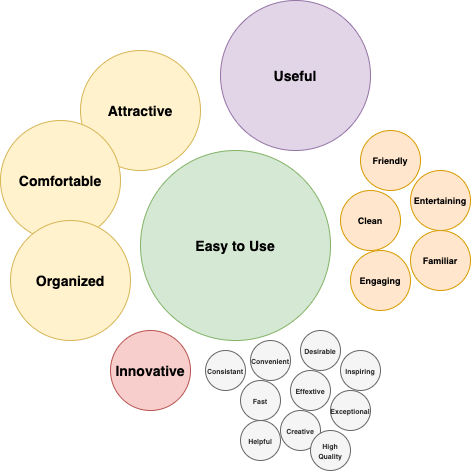
\includegraphics[width=0.8\textwidth]{./Images/wordcloud.png}
\caption{Generated word cloud from the most used terms to describe the Sterio system}
\label{fig:wordcloud}
\end{figure}

Finally, and most importantly, a final short interview was conducted with all participating users, which provided another way for the participants to share their experience in their own words, thus giving us more detailed and complete insight on their experience.

Most users noted that they would use the platform on a daily basis, while others said it would be particularly interesting to use on specific occasions (such as driving or cooking). They noted that the overall interface was very easy and quick to use, making the platform a very compelling complement to their audio media consuming routines. 

A vast majority of users felt they were listening to a 'real' radio station, noting also that they felt a connection in some way. When asked if they entangled a human element, and/or a connection with them in a similar way that traditional radio stations provide, all users replied affirmatively. One user pointed out that, by using the system, it could the weariness felt whilst using a music streaming service for a long periods of time. 

Regarding the used text-to-speech, the majority of users thought it was more natural and human-like than what they were expecting, but it still had some flaws when pronnouncing more complex words.

As for the social component of the platform, most users thought it was very well integrated and developed. They noted that they would like to expand their audio consuming social sharing habits, and that the currently available music streaming services are lacking this facet. One particular user suggested the integration of this social component with real radio stations, providing them a way to create and share pre-customized stations with real radio hosts interacting with the listener, but by combining a user's selection of music library, without compromising the customizable capabilities.

Finally, most users believed that this platform could be widley adopted by the community, as they found it very unique and desirable. In conjunction with the analyzed feedback, this assures that our goals were met successfully.

% #############################################################################
\section{Discussion}

Audio streaming services are used daily by millions worldwide, enabling on-demand listening and the discovery of songs, artists, and podcasts that closely align with the listener’s preferences. Meanwhile, traditional terrestrial radio persists as another ubiquitous and still viable mode of accessing more pre-programmed music and news content, including traffic reports and weather information. While both media services offer listeners a distinct set of value propositions, efforts to combine the 'best of both worlds' have been few and far between. After a background analysis in Chapters ~\ref{chap:relatedwork}, we set the goal of this project to answer to the question: "How can audio media consumers' music streaming and traditional terrestrial radio habits be best represented in an integrated and personalized experience that may be shared within small networks of friends and family?"

With both our user studies conducted in Chapters ~\ref{chap:userresearch} and ~\ref{sec:speeddating}, and with our hunt statement in mind, we described in Section ~\ref{sec:req} the requirements that a platform of this scope should have. In short, our ultimate goal was to design and develop a novel listening experience, dubbed Sterio, aimed at merging the best of both worlds — i.e. music streaming services and traditional terrestrial radio — in an interactive, user-centered, appealing, engaging, and innovative platform.

The future of radio has to blend the convenience and viability of music streaming services with the human touch and connection to the world that terrestrial radio stations provide. Sharing this personalized experience with friends and family is a must-have functionality, as the music plays a key role in users’ lives and we’re living in a social age where users want to be connected with each other. By merging a users' music streaming service library and audio dynamically generated from news, social networks, or even personal sources, with non-speech audio sound effects and background music, into a radio-like integrated, interactive and social experience, Sterio forms a new approach to ubiquitous audio consuming platforms. 

From the analysis of the results of the usability testing, we can conclude that our system had a phenomenal user acceptance and usability. This indicates that our platform has not only met user's needs and expectations but exceeded them. Thus, taking all into account, we consider that we've successfully met our goals, proving that the concept of interactive radio can indeed be further augmented into a novel, integrated experience for individual listeners and their close networks of family and friends.
